\documentclass[aspectratio=1610]{beamer}
\usepackage[utf8]{inputenc}
% \usepackage[default,oldstyle,scale=0.95]{opensans}
% \usepackage[T1]{fontenc}
\usepackage{sansmathfonts}
\usepackage[T1]{fontenc}

\usepackage[natbib=true,style=numeric,sorting=none]{biblatex}
\addbibresource{references.bib}

\usepackage{pgf-pie}  
\usepackage{caption}
\usepackage{subcaption}
\usepackage{algorithm}
\usepackage{algpseudocode}
\usepackage{amsmath,amssymb,amsfonts}
\usepackage{svg}

\usetikzlibrary{arrows.meta}
\usetikzlibrary{tikzmark}
\usetikzlibrary{math}
\usetikzlibrary{backgrounds,calc,positioning}
\usepackage{qrcode}
\usepackage{siunitx}
\usetikzlibrary{patterns,positioning,arrows.meta,decorations.pathreplacing}

\usepackage{pgfplots}



\usetheme{main}

\captionsetup{font=scriptsize,labelfont=scriptsize}


\title[Numerical optimization]{Numerical optimization : theory and applications}

\date[]{}
\author[AM]{\textbf{Ammar Mian} \\ \footnotesize Associate professor, LISTIC, Université Savoie Mont Blanc}

\newcommand{\red}[1]{\textcolor{red}{#1}}
% \newcommand{\alert}[1]{{\textbf{\alert{#1}}}}


%%%%%% NEW MATH DEFINITIONS %%%%%

\usepackage{amsmath,amsfonts,bm}

% Mark sections of captions for referring to divisions of figures
\newcommand{\figleft}{{\em (Left)}}
\newcommand{\figcenter}{{\em (Center)}}
\newcommand{\figright}{{\em (Right)}}
\newcommand{\figtop}{{\em (Top)}}
\newcommand{\figbottom}{{\em (Bottom)}}
\newcommand{\captiona}{{\em (a)}}
\newcommand{\captionb}{{\em (b)}}
\newcommand{\captionc}{{\em (c)}}
\newcommand{\captiond}{{\em (d)}}

% Highlight a newly defined term
\newcommand{\newterm}[1]{{\bf #1}}


% Figure reference, lower-case.
\def\figref#1{figure~\ref{#1}}
% Figure reference, capital. For start of sentence
\def\Figref#1{Figure~\ref{#1}}
\def\twofigref#1#2{figures \ref{#1} and \ref{#2}}
\def\quadfigref#1#2#3#4{figures \ref{#1}, \ref{#2}, \ref{#3} and \ref{#4}}
% Section reference, lower-case.
\def\secref#1{section~\ref{#1}}
% Section reference, capital.
\def\Secref#1{Section~\ref{#1}}
% Reference to two sections.
\def\twosecrefs#1#2{sections \ref{#1} and \ref{#2}}
% Reference to three sections.
\def\secrefs#1#2#3{sections \ref{#1}, \ref{#2} and \ref{#3}}
% Reference to an equation, lower-case.
% \def\eqref#1{equation~\ref{#1}}
% Reference to an equation, upper case
\def\Eqref#1{Equation~\ref{#1}}
% A raw reference to an equation---avoid using if possible
\def\plaineqref#1{\ref{#1}}
% Reference to a chapter, lower-case.
\def\chapref#1{chapter~\ref{#1}}
% Reference to an equation, upper case.
\def\Chapref#1{Chapter~\ref{#1}}
% Reference to a range of chapters
\def\rangechapref#1#2{chapters\ref{#1}--\ref{#2}}
% Reference to an algorithm, lower-case.
\def\algref#1{algorithm~\ref{#1}}
% Reference to an algorithm, upper case.
\def\Algref#1{Algorithm~\ref{#1}}
\def\twoalgref#1#2{algorithms \ref{#1} and \ref{#2}}
\def\Twoalgref#1#2{Algorithms \ref{#1} and \ref{#2}}
% Reference to a part, lower case
\def\partref#1{part~\ref{#1}}
% Reference to a part, upper case
\def\Partref#1{Part~\ref{#1}}
\def\twopartref#1#2{parts \ref{#1} and \ref{#2}}

\def\ceil#1{\lceil #1 \rceil}
\def\floor#1{\lfloor #1 \rfloor}
\def\1{\bm{1}}
\newcommand{\train}{\mathcal{D}}
\newcommand{\valid}{\mathcal{D_{\mathrm{valid}}}}
\newcommand{\test}{\mathcal{D_{\mathrm{test}}}}

\def\eps{{\epsilon}}


% Random variables
\def\reta{{\textnormal{$\eta$}}}
\def\ra{{\textnormal{a}}}
\def\rb{{\textnormal{b}}}
\def\rc{{\textnormal{c}}}
\def\rd{{\textnormal{d}}}
\def\re{{\textnormal{e}}}
\def\rf{{\textnormal{f}}}
\def\rg{{\textnormal{g}}}
\def\rh{{\textnormal{h}}}
\def\ri{{\textnormal{i}}}
\def\rj{{\textnormal{j}}}
\def\rk{{\textnormal{k}}}
\def\rl{{\textnormal{l}}}
% rm is already a command, just don't name any random variables m
\def\rn{{\textnormal{n}}}
\def\ro{{\textnormal{o}}}
\def\rp{{\textnormal{p}}}
\def\rq{{\textnormal{q}}}
\def\rr{{\textnormal{r}}}
\def\rs{{\textnormal{s}}}
\def\rt{{\textnormal{t}}}
\def\ru{{\textnormal{u}}}
\def\rv{{\textnormal{v}}}
\def\rw{{\textnormal{w}}}
\def\rx{{\textnormal{x}}}
\def\ry{{\textnormal{y}}}
\def\rz{{\textnormal{z}}}

% Random vectors
\def\rvepsilon{{\mathbf{\epsilon}}}
\def\rvtheta{{\mathbf{\theta}}}
\def\rva{{\mathbf{a}}}
\def\rvb{{\mathbf{b}}}
\def\rvc{{\mathbf{c}}}
\def\rvd{{\mathbf{d}}}
\def\rve{{\mathbf{e}}}
\def\rvf{{\mathbf{f}}}
\def\rvg{{\mathbf{g}}}
\def\rvh{{\mathbf{h}}}
\def\rvu{{\mathbf{i}}}
\def\rvj{{\mathbf{j}}}
\def\rvk{{\mathbf{k}}}
\def\rvl{{\mathbf{l}}}
\def\rvm{{\mathbf{m}}}
\def\rvn{{\mathbf{n}}}
\def\rvo{{\mathbf{o}}}
\def\rvp{{\mathbf{p}}}
\def\rvq{{\mathbf{q}}}
\def\rvr{{\mathbf{r}}}
\def\rvs{{\mathbf{s}}}
\def\rvt{{\mathbf{t}}}
\def\rvu{{\mathbf{u}}}
\def\rvv{{\mathbf{v}}}
\def\rvw{{\mathbf{w}}}
\def\rvx{{\mathbf{x}}}
\def\rvy{{\mathbf{y}}}
\def\rvz{{\mathbf{z}}}

% Elements of random vectors
\def\erva{{\textnormal{a}}}
\def\ervb{{\textnormal{b}}}
\def\ervc{{\textnormal{c}}}
\def\ervd{{\textnormal{d}}}
\def\erve{{\textnormal{e}}}
\def\ervf{{\textnormal{f}}}
\def\ervg{{\textnormal{g}}}
\def\ervh{{\textnormal{h}}}
\def\ervi{{\textnormal{i}}}
\def\ervj{{\textnormal{j}}}
\def\ervk{{\textnormal{k}}}
\def\ervl{{\textnormal{l}}}
\def\ervm{{\textnormal{m}}}
\def\ervn{{\textnormal{n}}}
\def\ervo{{\textnormal{o}}}
\def\ervp{{\textnormal{p}}}
\def\ervq{{\textnormal{q}}}
\def\ervr{{\textnormal{r}}}
\def\ervs{{\textnormal{s}}}
\def\ervt{{\textnormal{t}}}
\def\ervu{{\textnormal{u}}}
\def\ervv{{\textnormal{v}}}
\def\ervw{{\textnormal{w}}}
\def\ervx{{\textnormal{x}}}
\def\ervy{{\textnormal{y}}}
\def\ervz{{\textnormal{z}}}

% Random matrices
\def\rmA{{\mathbf{A}}}
\def\rmB{{\mathbf{B}}}
\def\rmC{{\mathbf{C}}}
\def\rmD{{\mathbf{D}}}
\def\rmE{{\mathbf{E}}}
\def\rmF{{\mathbf{F}}}
\def\rmG{{\mathbf{G}}}
\def\rmH{{\mathbf{H}}}
\def\rmI{{\mathbf{I}}}
\def\rmJ{{\mathbf{J}}}
\def\rmK{{\mathbf{K}}}
\def\rmL{{\mathbf{L}}}
\def\rmM{{\mathbf{M}}}
\def\rmN{{\mathbf{N}}}
\def\rmO{{\mathbf{O}}}
\def\rmP{{\mathbf{P}}}
\def\rmQ{{\mathbf{Q}}}
\def\rmR{{\mathbf{R}}}
\def\rmS{{\mathbf{S}}}
\def\rmT{{\mathbf{T}}}
\def\rmU{{\mathbf{U}}}
\def\rmV{{\mathbf{V}}}
\def\rmW{{\mathbf{W}}}
\def\rmX{{\mathbf{X}}}
\def\rmY{{\mathbf{Y}}}
\def\rmZ{{\mathbf{Z}}}

% Elements of random matrices
\def\ermA{{\textnormal{A}}}
\def\ermB{{\textnormal{B}}}
\def\ermC{{\textnormal{C}}}
\def\ermD{{\textnormal{D}}}
\def\ermE{{\textnormal{E}}}
\def\ermF{{\textnormal{F}}}
\def\ermG{{\textnormal{G}}}
\def\ermH{{\textnormal{H}}}
\def\ermI{{\textnormal{I}}}
\def\ermJ{{\textnormal{J}}}
\def\ermK{{\textnormal{K}}}
\def\ermL{{\textnormal{L}}}
\def\ermM{{\textnormal{M}}}
\def\ermN{{\textnormal{N}}}
\def\ermO{{\textnormal{O}}}
\def\ermP{{\textnormal{P}}}
\def\ermQ{{\textnormal{Q}}}
\def\ermR{{\textnormal{R}}}
\def\ermS{{\textnormal{S}}}
\def\ermT{{\textnormal{T}}}
\def\ermU{{\textnormal{U}}}
\def\ermV{{\textnormal{V}}}
\def\ermW{{\textnormal{W}}}
\def\ermX{{\textnormal{X}}}
\def\ermY{{\textnormal{Y}}}
\def\ermZ{{\textnormal{Z}}}

% Vectors
\def\vzero{{\bm{0}}}
\def\vone{{\bm{1}}}
\def\vmu{{\bm{\mu}}}
\def\vtheta{{\bm{\theta}}}
\def\va{{\bm{a}}}
\def\vb{{\bm{b}}}
\def\vc{{\bm{c}}}
\def\vd{{\bm{d}}}
\def\ve{{\bm{e}}}
\def\vf{{\bm{f}}}
\def\vg{{\bm{g}}}
\def\vh{{\bm{h}}}
\def\vi{{\bm{i}}}
\def\vj{{\bm{j}}}
\def\vk{{\bm{k}}}
\def\vl{{\bm{l}}}
\def\vm{{\bm{m}}}
\def\vn{{\bm{n}}}
\def\vo{{\bm{o}}}
\def\vp{{\bm{p}}}
\def\vq{{\bm{q}}}
\def\vr{{\bm{r}}}
\def\vs{{\bm{s}}}
\def\vt{{\bm{t}}}
\def\vu{{\bm{u}}}
\def\vv{{\bm{v}}}
\def\vw{{\bm{w}}}
\def\vx{{\bm{x}}}
\def\vy{{\bm{y}}}
\def\vz{{\bm{z}}}

% Elements of vectors
\def\evalpha{{\alpha}}
\def\evbeta{{\beta}}
\def\evepsilon{{\epsilon}}
\def\evlambda{{\lambda}}
\def\evomega{{\omega}}
\def\evmu{{\mu}}
\def\evpsi{{\psi}}
\def\evsigma{{\sigma}}
\def\evtheta{{\theta}}
\def\eva{{a}}
\def\evb{{b}}
\def\evc{{c}}
\def\evd{{d}}
\def\eve{{e}}
\def\evf{{f}}
\def\evg{{g}}
\def\evh{{h}}
\def\evi{{i}}
\def\evj{{j}}
\def\evk{{k}}
\def\evl{{l}}
\def\evm{{m}}
\def\evn{{n}}
\def\evo{{o}}
\def\evp{{p}}
\def\evq{{q}}
\def\evr{{r}}
\def\evs{{s}}
\def\evt{{t}}
\def\evu{{u}}
\def\evv{{v}}
\def\evw{{w}}
\def\evx{{x}}
\def\evy{{y}}
\def\evz{{z}}

% Matrix
\def\mA{{\bm{A}}}
\def\mB{{\bm{B}}}
\def\mC{{\bm{C}}}
\def\mD{{\bm{D}}}
\def\mE{{\bm{E}}}
\def\mF{{\bm{F}}}
\def\mG{{\bm{G}}}
\def\mH{{\bm{H}}}
\def\mI{{\bm{I}}}
\def\mJ{{\bm{J}}}
\def\mK{{\bm{K}}}
\def\mL{{\bm{L}}}
\def\mM{{\bm{M}}}
\def\mN{{\bm{N}}}
\def\mO{{\bm{O}}}
\def\mP{{\bm{P}}}
\def\mQ{{\bm{Q}}}
\def\mR{{\bm{R}}}
\def\mS{{\bm{S}}}
\def\mT{{\bm{T}}}
\def\mU{{\bm{U}}}
\def\mV{{\bm{V}}}
\def\mW{{\bm{W}}}
\def\mX{{\bm{X}}}
\def\mY{{\bm{Y}}}
\def\mZ{{\bm{Z}}}
\def\mBeta{{\bm{\beta}}}
\def\mPhi{{\bm{\Phi}}}
\def\mLambda{{\bm{\Lambda}}}
\def\mSigma{{\bm{\Sigma}}}

% Tensor
\DeclareMathAlphabet{\mathsfit}{\encodingdefault}{\sfdefault}{m}{sl}
\SetMathAlphabet{\mathsfit}{bold}{\encodingdefault}{\sfdefault}{bx}{n}
\newcommand{\tens}[1]{\bm{\mathsfit{#1}}}
\def\tA{{\tens{A}}}
\def\tB{{\tens{B}}}
\def\tC{{\tens{C}}}
\def\tD{{\tens{D}}}
\def\tE{{\tens{E}}}
\def\tF{{\tens{F}}}
\def\tG{{\tens{G}}}
\def\tH{{\tens{H}}}
\def\tI{{\tens{I}}}
\def\tJ{{\tens{J}}}
\def\tK{{\tens{K}}}
\def\tL{{\tens{L}}}
\def\tM{{\tens{M}}}
\def\tN{{\tens{N}}}
\def\tO{{\tens{O}}}
\def\tP{{\tens{P}}}
\def\tQ{{\tens{Q}}}
\def\tR{{\tens{R}}}
\def\tS{{\tens{S}}}
\def\tT{{\tens{T}}}
\def\tU{{\tens{U}}}
\def\tV{{\tens{V}}}
\def\tW{{\tens{W}}}
\def\tX{{\tens{X}}}
\def\tY{{\tens{Y}}}
\def\tZ{{\tens{Z}}}


% Graph
\def\gA{{\mathcal{A}}}
\def\gB{{\mathcal{B}}}
\def\gC{{\mathcal{C}}}
\def\gD{{\mathcal{D}}}
\def\gE{{\mathcal{E}}}
\def\gF{{\mathcal{F}}}
\def\gG{{\mathcal{G}}}
\def\gH{{\mathcal{H}}}
\def\gI{{\mathcal{I}}}
\def\gJ{{\mathcal{J}}}
\def\gK{{\mathcal{K}}}
\def\gL{{\mathcal{L}}}
\def\gM{{\mathcal{M}}}
\def\gN{{\mathcal{N}}}
\def\gO{{\mathcal{O}}}
\def\gP{{\mathcal{P}}}
\def\gQ{{\mathcal{Q}}}
\def\gR{{\mathcal{R}}}
\def\gS{{\mathcal{S}}}
\def\gT{{\mathcal{T}}}
\def\gU{{\mathcal{U}}}
\def\gV{{\mathcal{V}}}
\def\gW{{\mathcal{W}}}
\def\gX{{\mathcal{X}}}
\def\gY{{\mathcal{Y}}}
\def\gZ{{\mathcal{Z}}}

% Sets
\def\sA{{\mathbb{A}}}
\def\sB{{\mathbb{B}}}
\def\sC{{\mathbb{C}}}
\def\sD{{\mathbb{D}}}
% Don't use a set called E, because this would be the same as our symbol
% for expectation.
\def\sF{{\mathbb{F}}}
\def\sG{{\mathbb{G}}}
\def\sH{{\mathbb{H}}}
\def\sI{{\mathbb{I}}}
\def\sJ{{\mathbb{J}}}
\def\sK{{\mathbb{K}}}
\def\sL{{\mathbb{L}}}
\def\sM{{\mathbb{M}}}
\def\sN{{\mathbb{N}}}
\def\sO{{\mathbb{O}}}
\def\sP{{\mathbb{P}}}
\def\sQ{{\mathbb{Q}}}
\def\sR{{\mathbb{R}}}
\def\sS{{\mathbb{S}}}
\def\sT{{\mathbb{T}}}
\def\sU{{\mathbb{U}}}
\def\sV{{\mathbb{V}}}
\def\sW{{\mathbb{W}}}
\def\sX{{\mathbb{X}}}
\def\sY{{\mathbb{Y}}}
\def\sZ{{\mathbb{Z}}}

% Entries of a matrix
\def\emLambda{{\Lambda}}
\def\emA{{A}}
\def\emB{{B}}
\def\emC{{C}}
\def\emD{{D}}
\def\emE{{E}}
\def\emF{{F}}
\def\emG{{G}}
\def\emH{{H}}
\def\emI{{I}}
\def\emJ{{J}}
\def\emK{{K}}
\def\emL{{L}}
\def\emM{{M}}
\def\emN{{N}}
\def\emO{{O}}
\def\emP{{P}}
\def\emQ{{Q}}
\def\emR{{R}}
\def\emS{{S}}
\def\emT{{T}}
\def\emU{{U}}
\def\emV{{V}}
\def\emW{{W}}
\def\emX{{X}}
\def\emY{{Y}}
\def\emZ{{Z}}
\def\emSigma{{\Sigma}}

% entries of a tensor
% Same font as tensor, without \bm wrapper
\newcommand{\etens}[1]{\mathsfit{#1}}
\def\etLambda{{\etens{\Lambda}}}
\def\etA{{\etens{A}}}
\def\etB{{\etens{B}}}
\def\etC{{\etens{C}}}
\def\etD{{\etens{D}}}
\def\etE{{\etens{E}}}
\def\etF{{\etens{F}}}
\def\etG{{\etens{G}}}
\def\etH{{\etens{H}}}
\def\etI{{\etens{I}}}
\def\etJ{{\etens{J}}}
\def\etK{{\etens{K}}}
\def\etL{{\etens{L}}}
\def\etM{{\etens{M}}}
\def\etN{{\etens{N}}}
\def\etO{{\etens{O}}}
\def\etP{{\etens{P}}}
\def\etQ{{\etens{Q}}}
\def\etR{{\etens{R}}}
\def\etS{{\etens{S}}}
\def\etT{{\etens{T}}}
\def\etU{{\etens{U}}}
\def\etV{{\etens{V}}}
\def\etW{{\etens{W}}}
\def\etX{{\etens{X}}}
\def\etY{{\etens{Y}}}
\def\etZ{{\etens{Z}}}

% The true underlying data generating distribution
\newcommand{\pdata}{p_{\rm{data}}}
% The empirical distribution defined by the training set
\newcommand{\ptrain}{\hat{p}_{\rm{data}}}
\newcommand{\Ptrain}{\hat{P}_{\rm{data}}}
% The model distribution
\newcommand{\pmodel}{p_{\rm{model}}}
\newcommand{\Pmodel}{P_{\rm{model}}}
\newcommand{\ptildemodel}{\tilde{p}_{\rm{model}}}
% Stochastic autoencoder distributions
\newcommand{\pencode}{p_{\rm{encoder}}}
\newcommand{\pdecode}{p_{\rm{decoder}}}
\newcommand{\precons}{p_{\rm{reconstruct}}}

\newcommand{\laplace}{\mathrm{Laplace}} % Laplace distribution

\newcommand{\E}{\mathbb{E}}
\newcommand{\Ls}{\mathcal{L}}
% \newcommand{\R}{\mathbb{R}}
\newcommand{\emp}{\tilde{p}}
\newcommand{\lr}{\alpha}
\newcommand{\reg}{\lambda}
\newcommand{\rect}{\mathrm{rectifier}}
\newcommand{\softmax}{\mathrm{softmax}}
\newcommand{\sigmoid}{\sigma}
\newcommand{\softplus}{\zeta}
\newcommand{\KL}{D_{\mathrm{KL}}}
\newcommand{\Var}{\mathrm{Var}}
\newcommand{\standarderror}{\mathrm{SE}}
\newcommand{\Cov}{\mathrm{Cov}}
% Wolfram Mathworld says $L^2$ is for function spaces and $\ell^2$ is for vectors
% But then they seem to use $L^2$ for vectors throughout the site, and so does
% wikipedia.
\newcommand{\normlzero}{L^0}
\newcommand{\normlone}{L^1}
\newcommand{\normltwo}{L^2}
\newcommand{\normlp}{L^p}
\newcommand{\normmax}{L^\infty}

\newcommand{\parents}{Pa} % See usage in notation.tex. Chosen to match Daphne's book.

% \DeclareMathOperator*{\argmax}{arg\,max}
% \DeclareMathOperator*{\argmin}{arg\,min}

\DeclareMathOperator{\sign}{sign}
\DeclareMathOperator{\Tr}{Tr}
\let\ab\allowbreak


\newcommand{\mat}[1]{\mathbf{#1}}
\renewcommand{\vec}[1]{\boldsymbol{#1}}
\renewcommand{\det}[1]{\lvert #1 \rvert}
\newcommand{\Esp}[2]{\mathbb{E}_{#1}\left[#2 \right]}
\renewcommand{\v}{\vec{v}}
\newcommand{\eye}[1]{\mathbf{I}_{#1}}
\newcommand{\norm}[1]{\left\| #1 \right\|}
\newcommand{\argmin}[1]{\underset{#1}{\operatorname{argmin}}}
\newcommand{\argmax}[1]{\underset{#1}{\operatorname{argmax}}}

% \newcommand{\bm}[1]{\boldsymbol{#1}}
\def\R{{\mathbb{R}}}
\def\K{{\mathbb{K}}}
\def\C{{\mathbb{C}}}
\def\N{{\mathbb{N}}}
\def\Z{{\mathbb{Z}}}
\def\d{{\rm d}}


\def\eme{{{\grave{e}me}}}

\def\m{{\mbox{m}}}
\def\Hz{{\mbox{Hz}}}
\def\Watt{{\mbox{W}}}

\DeclareMathOperator{\vecop}{vec}
\DeclareMathOperator{\unvec}{vec^{-1}}
\DeclareMathOperator{\tr}{tr}
\DeclareMathOperator{\diag}{diag}
\DeclareMathOperator{\prox}{prox}
\DeclareMathOperator{\rank}{rank}
\DeclareMathOperator{\complexj}{\mathsf{j}}
\DeclareMathOperator{\proj}{proj}
\DeclareMathOperator{\sinc}{sinc}






\AtBeginBibliography{\scriptsize}

%%%%%%%%%%%%%%%%%%%%%%%%%%%%%%%%%%%%%%%%%%%%%%%%%%%%%%%%%%%%
%                     END OF PREAMBLE
%
%%%%%%%%%%%%%%%%%%%%%%%%%%%%%%%%%%%%%%%%%%%%%%%%%%%%%%%%%%%%

\begin{document}
%%%%%%%%%%%%%%%


  
\begin{frame}[noframenumbering,plain]
\titlepage
\end{frame}
\begingroup
\setbeamercolor{background canvas}{bg=main}
\setbeamercolor{titlelike}{fg=text-light, bg=light}
\begin{frame}[noframenumbering,plain]{Outline}
    \tableofcontents[]
\end{frame}

\endgroup

\AtBeginSection[]{
        \setbeamercolor{background canvas}{bg=main} 
    \begin{frame}[plain, noframenumbering]
        \tableofcontents[currentsection]
    \end{frame}
    \setbeamercolor{background canvas}{bg=light} 
}


\AtBeginSubsection[]
{
    \setbeamercolor{background canvas}{bg=main} 
    \begin{frame}[noframenumbering, plain, label=]
        % \frametitle{Plan}  
        \tableofcontents[currentsection,currentsubsection]
    \end{frame}
    \setbeamercolor{background canvas}{bg=light} 
}



%%%%%%%%%%%%%%%%%%%%%%%%%%%%%%%%%%%%%%%%%%%%%%%%%%%%%%%%%%%%
%%%%%%%%%%%%%%%%%%%%%%%%%%%%%%%%%%%%%%%%%%%%%%%%%%%%%%%%%%%%


\section{Introduction}

\subsection{Course organization}

\begin{frame}{Online ressources}

  The syllabus, course monograph and slides are available at:

  \medskip

  \begin{figure}[h]
    \qrcode[height=1.5in] {https://ammarmian.github.io/numerical_optimization/}
  \end{figure}

\end{frame}

\begin{frame}{Book ressources}
  \begin{block}{Main book}
    \fullcite{nocedal1999numerical}
  \end{block}
  \begin{block}{Additional in convex optimization}
    \fullcite{boyd2004convex}
  \end{block}
  \begin{block}{For reminders}
    \fullcite{magnus2019matrix}
  \end{block}
\end{frame}

\begin{frame}{Part I - Fundamentals}

  \textbf{Oranisation of first week}
  \begin{table}[h]
\resizebox{\textwidth}{!}{%
\begin{tabular}{lllll}
Session & Duration & Content                                                                   & Date               & Room  \\
\hline
CM1     & 1.5h     & Introduction, Linear algebra and Differentiation reminders, and exercices & 2 June 2025 10am   & B-120 \\
CM2     & 1.5h     & Steepest descent algorithm, Newton method and convexity                   & 2 June 2025 1.15pm & B-120 \\
TD1     & 1.5h     & Application to linear regression                                          & 2 June 2025 3pm    & C-213 \\
CM3     & 1.5h     & Linesearch algorithms and their convergence                               & 3 June 2025 10am   & B-120 \\
CM4     & 1.5h     & Constrained optimization : linear programming and lagrangian methods      & 3 June 2025 1.15pm & B-120 \\
TD2     & 1.5h     & Implementation of Linesearch methods                                      & 3 June 2025 3pm    & C-213
\end{tabular}
  }

  \medskip

  Then on 5 June 2025 at 1pm, a project on Implementation of inverse problems for image processing, by \emph{Yassine Mhiri}.
\end{table}
  
\end{frame}

\subsection{The setup}
\begin{frame}{Numerical optimization}

  What is this course about ?

  \pause

  \begin{block}{Numerical optimization}
    Numerical optimization is the computational process of finding the best solution to a mathematical problem when analytical (exact) methods are impractical or impossible.
  \end{block}


  What problem ? 
  \pause

  \begin{itemize}
    \item \textbf{Variables : } $\mathbf{x}_1$, $\dots$, $\mathbf{x}_d$ organised as $\mathbf{x}\in\mathbb{R}^d$
    \item \textbf{Objective function:} $f:\mathcal{X}\subset\mathbb{R}^d \mapsto \mathbb{R}$
    \item \textbf{Constraints :} $\mathcal{S} = \{\mathbf{x}\in\mathcal{X} : h_{1,\dots,p}(\mathbf{x})=0,\, g_{1,\dots,q}(\mathbf{x})\geq 0\}$
  \end{itemize}


\end{frame}

\begin{frame}{Practical examples (1/3)}
  
  \begin{figure}
    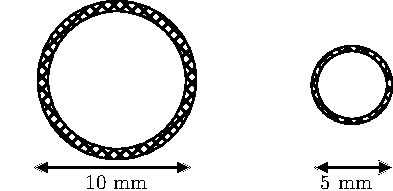
\includegraphics[height=2cm]{figures/cables.pdf}
  \end{figure}

  \begin{block}{Cable factory}
    \small
    A factory produces copper cables of 5mm and 10mm diameter, on which the profit is respectively 2 and 7 euros per meter. The copper available to the factory allows for the production of 20 km of 5mm diameter cable per week. The production of 10mm cable requires 4 times more copper than that of 5mm cable. For demand reasons, the weekly production of 5mm cable must not exceed 15 km, and for logistical reasons, the production of 10mm cable must not represent more than 40\% of the total production.
  \end{block}
  \pause

  $\rightarrow$ How to know what is the most profitable setup ?

\end{frame}


\begin{frame}{Practical exmaples (2/3)}

  \begin{block}{Image denoising}
    \begin{figure}[h]
      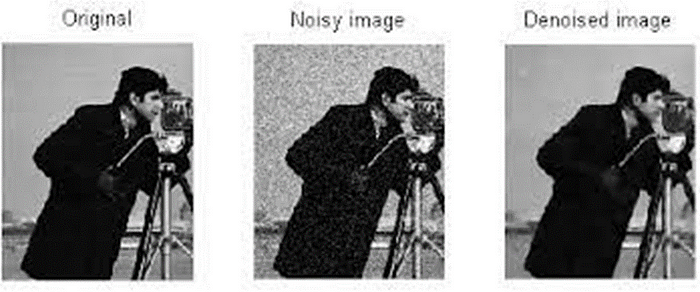
\includegraphics[height=3cm]{figures/denoising.png}
    \end{figure}

  \end{block}
  
    \pause  

    $\rightarrow$ How to model the wanted signal and then find the best one among all possible signals ?
\end{frame}

\begin{frame}{Practical examples (3/3)}
  \begin{block}{Portfolio optimization}
    \small
    An investor has \$1M to allocate between 3 assets: stocks (expected return 8\%, risk 15\%), bonds (expected return 4\%, risk 5\%), and real estate (expected return 6\%, risk 10\%). The correlations between assets are: stocks-bonds = 0.2, stocks-real estate = 0.3, bonds-real estate = 0.1. The investor wants to maximize expected return while keeping portfolio risk below 8\%.
  \end{block}
  \pause
  
  \vspace{0.3cm}
  \textbf{Mathematical formulation:}
  \begin{equation}
    \max_{\mathbf{w}} \quad  \sum_{i=1}^{3} w_i \mu_i 
    s.t \quad \sqrt{\mathbf{w}^\mathrm{T} \boldsymbol{\Sigma} \mathbf{w}} \leq 0.08,\, \sum_{i=1}^{3} w_i = 1,\, w_i \geq 0, \quad i = 1,2,3
  \end{equation}
  
  where $w_i$ = weight in asset $i$, $\mu_i$ = expected return, $\Sigma$ = covariance matrix
  
  \pause
  $\rightarrow$ How to find the optimal balance between risk and return?
\end{frame}


\section{Linear Algebra}

\subsection{Vectors and matrices}

\begin{frame}{Notations}
  \begin{block}{Matrix vectors, and scalars}
    \begin{itemize}
      \item Scalars $\in\mathbb{R}$ are lowercase letters: $x,y,z$ or greek letters: $\alpha, \beta, \gamma$
      \item Vectors $\in\mathbb{R}^d$ are lowercase bold letters: $\mathbf{x}, \mathbf{y}, \mathbf{z}$ or greek letters: $\boldsymbol{\theta}$
      \item Matrices $\in\mathbb{R}^{m,n}$ are uppercase bold letters: $\mathbf{X}, \mathbf{Y}, \mathbf{Z}$ 
    \end{itemize}
    > We don't consider data in $\mathbb{C}^d$ but it could be treated with equivalence $\mathbb{C}^d \equiv \mathbb{R}^{2d}$.
  \end{block}
  
  We also consider functions:
  {\footnotesize
  \begin{itemize}
    \item $f:\mathbb{R}^d\to\mathbb{R}$ is a function from $\mathbb{R}^d$ to $\mathbb{R}$, e.g. $f(\mathbf{x}) = \mathbf{x}^\mathrm{T}\mathbf{A}\mathbf{x} + \mathbf{b}^\mathrm{T}\mathbf{x} + c$
    \item $g:\mathbb{R}^{m,n}\to\mathbb{R}$ is a function from $\mathbb{R}^{m,n}$ to $\mathbb{R}$, e.g. $g(\mathbf{X}) = \|\mathbf{X}\|_F^2$
    \item $h:\mathbb{R}^d\to\mathbb{R}^p$ is a function from $\mathbb{R}^d$ to $\mathbb{R}^p$, e.g. $h(\mathbf{x}) = [x_1^2, x_2^2, \ldots, x_d^2]^\mathrm{T}$
    \item $l:\mathbb{R}^{m,n}\to\mathbb{R}^q$ is a function from $\mathbb{R}^{m,n}$ to $\mathbb{R}^q$, e.g. $l(\mathbf{X}) = \begin{pmatrix} X_{11}^2 \\ X_{12}^2 \\ \vdots \\ X_{mn}^2 \end{pmatrix}$
  \end{itemize}
  }
\end{frame}

\begin{frame}{Vectors}
  \begin{block}{Usual operations}
    \begin{itemize}
      \item Sum: $\mathbf{x} + \mathbf{y} = \begin{pmatrix} x_1 + y_1 \\ x_2 + y_2 \\ \vdots \\ x_d + y_d \end{pmatrix}$
      \item Scalar product: $\mathbf{x}^\mathrm{T}\mathbf{y} = x_1 y_1 + x_2 y_2 + \dots + x_d y_d$
      \item $p$-norm: $\|\mathbf{x}\|_p = \left(\sum_{i=1}^d |x_i|^p\right)^{1/p}$, with $\|\mathbf{x}\|_2 = \sqrt{\mathbf{x}^\mathrm{T}\mathbf{x}}$
    \end{itemize}
  \end{block}
\end{frame}

\begin{frame}{Vector spaces}

  \begin{block}{Span and Subspace}
    For a set of vectors $\{\mathbf{v}_1, \ldots, \mathbf{v}_k\}$:
    $
      \mathrm{span}(\{\mathbf{v}_1, \ldots, \mathbf{v}_k\}) = \left\{ c_1\mathbf{v}_1 + c_2\mathbf{v}_2 + \ldots + c_k\mathbf{v}_k : c_i \in \mathbb{R} \right\}
    $.

    A subspace is a subset of a vector space that is closed under addition and scalar multiplication.
  \end{block}

  \begin{block}{Linear independence}
    A set of vectors $\{\mathbf{v}_1, \ldots, \mathbf{v}_k\}$ is said to be \textbf{linearly independent} if the only solution to the equation $c_1\mathbf{v}_1 + c_2\mathbf{v}_2 + \ldots + c_k\mathbf{v}_k = \mathbf{0}$ is $c_1 = c_2 = \ldots = c_k = 0$.
  \end{block}

  \textbf{Basis}: A set of vectors $\{\mathbf{b}_1, \ldots, \mathbf{b}_k\}$ is a \textbf{basis} of a vector space if they are linearly independent and span the space. 
\end{frame}

\begin{frame}{Matrices}
  \begin{block}{Usual operations}
    \begin{itemize}
      \item Sum for $\mathbf{X},\mathbf{Y}\in\mathbb{R}^{m,n}$: $\mathbf{X} + \mathbf{Y} = \mathbf{Z}\in\mathbb{R}^{m,n}$ with $Z_{ij} = X_{ij} + Y_{ij}$ for $i=1,\dots,m$ and $j=1,\dots,n$
      \item Hadamard product for $\mathbf{X},\mathbf{Y}\in\mathbb{R}^{m,n}$: $\mathbf{X}\circ\mathbf{Y} = \mathbf{Z}\in\mathbb{R}^{m,n}$ with $Z_{ij} = X_{ij}Y_{ij}$ for $i=1,\dots,m$ and $j=1,\dots,n$
      \item Matrix multiplication for $\mathbf{A}\in\mathbb{R}^{m,n}$, $\mathbf{B}\in\mathbb{R}^{n,p}$: $\mathbf{A}\mathbf{B}=\mathbf{C}\in\mathbb{R}^{m,p}$ with $C_{ij} = \sum_{k=1}^n A_{ik}B_{kj}$, for $i=1,\dots,m$ and $j=1,\dots,p$
      \item Frobenius norm: $\|\mathbf{X}\|_F = \sqrt{\sum\limits_i\sum\limits_j |X_{ij}|^2}$, with $\|\mathbf{X}\|_F^2 = \mathrm{Tr}\left(\mathbf{X}\circ\mathbf{X}\right)$
    \end{itemize}
  \end{block}

  Matrix/vector multiplication: for $\mathbf{A}\in\mathbb{R}^{m,n}$ and $\mathbf{x}\in\mathbb{R}^n$, we have $\mathbf{A}\mathbf{x} = \mathbf{y}\in\mathbb{R}^m$ with $y_i = \sum_{j=1}^n A_{ij}x_j$, for $i=1,\dots,m$.
\end{frame}

\begin{frame}{Matrices as linear applications}

  Given a basis in a vector space $\mathcal{V}$, a matrix $\mathbf{A}\in\mathbb{R}^{m,n}$ can be seen as a linear application $\mathcal{A}:\mathcal{V}\to\mathbb{R}^m$ such that for any vector $\mathbf{x}\in\mathcal{V}$, we have:
    % Matrix vecotr product with basis e_i and showing that each element of V = \sum_{i=1}^n x_i e_i and thus Ax = A(\sum_{i=1}^n x_i e_i) = \sum_{i=1}^n x_i A e_i
    
    $\mathbf{x} = \sum_{i=1}^n x_i \mathbf{e}_i \Rightarrow$

    $$\mathcal{A}(\mathbf{x}) = \mathbf{A}\mathbf{x} = \sum_{i=1}^n x_i \mathcal{A}(\mathbf{e}_i) = \sum_{i=1}^n x_i \mathbf{a}_i, $$
    where $\mathbf{a}_i$ is the $i$-th column of $\mathbf{A}$.
\end{frame}

\begin{frame}{Matrix properties (1/2)}

  \begin{block}{Transpose}
    The transpose of a matrix $\mathbf{A}\in\mathbb{R}^{m,n}$ is denoted $\mathbf{A}^\mathrm{T}\in\mathbb{R}^{n,m}$ and is defined as $(\mathbf{A}^\mathrm{T})_{ij} = A_{ji}$.
  \end{block}

  \begin{block}{Symmetric matrices}
    A matrix $\mathbf{A}\in\mathbb{R}^{n,n}$ is symmetric if $\mathbf{A} = \mathbf{A}^\mathrm{T}$.
  \end{block}

  \begin{block}{Positive definite matrices}
    A symmetric matrix $\mathbf{A}\in\mathbb{R}^{n,n}$ is positive definite if for all non-zero vectors $\mathbf{x}\in\mathbb{R}^n$, we have $\mathbf{x}^\mathrm{T}\mathbf{A}\mathbf{x} > 0$.
  \end{block}
\end{frame}

\begin{frame}{Matrix properties (2/2)}

  \begin{block}{Inverse}
    The inverse of a square matrix $\mathbf{A}\in\mathbb{R}^{n,n}$ is denoted $\mathbf{A}^{-1}$ and is defined such that $\mathbf{A}\mathbf{A}^{-1} = \mathbf{I}_n$, where $\mathbf{I}_n$ is the identity matrix of size $n$.
  \end{block}

  \begin{block}{Determinant}
    The determinant of a square matrix $\mathbf{A}\in\mathbb{R}^{n,n}$ is denoted $\mathrm{det}(\mathbf{A})$ or $|\mathbf{A}|$ and is a scalar value that provides information about the matrix, such as whether it is invertible.
  \end{block}

  \begin{block}{Trace}
    The trace of a square matrix $\mathbf{A}\in\mathbb{R}^{n,n}$ is denoted $\mathrm{Tr}(\mathbf{A})$ and is defined as the sum of the diagonal elements: $\mathrm{Tr}(\mathbf{A}) = \sum_{i=1}^n A_{ii}$.
  \end{block}

\end{frame}


\begin{frame}{Exercices}
  TODO
\end{frame}



\subsection{Matrix decompositions}

\begin{frame}{Eigenvalues and eigenvectors}

  \begin{block}{Eigenvalues and eigenvectors}
    For a square matrix $\mathbf{A}\in\mathbb{R}^{n,n}$, a scalar $\lambda$ is an \textbf{eigenvalue} and a non-zero vector $\mathbf{v}\in\mathbb{R}^n$ is an \textbf{eigenvector} if they satisfy the equation:
    $$\mathbf{A}\mathbf{v} = \lambda \mathbf{v}.$$
  \end{block}

  \textbf{Computing eigenvalues and eigenvectors:} The eigenvalues of a matrix $\mathbf{A}$ are the roots of the characteristic polynomial $\mathrm{det}(\mathbf{A} - \lambda \mathbf{I}_n) = 0$, where $\mathbf{I}_n$ is the identity matrix of size $n$.


  \begin{block}{Spectral theorem}
    If $\mathbf{A}$ is symmetric, then it has $n$ real eigenvalues and $n$ orthogonal eigenvectors (i.e if $\mathbf{u}_i$ and $\mathbf{u}_j$ are eigenvectors of $\mathbf{A}$, then $\mathbf{u}_i^\mathrm{T}\mathbf{u}_j = 0$ for $i\neq j$).
  \end{block}
\end{frame}


\begin{frame}{Eigenvalue decomposition}

  \begin{block}{Eigenvalue decomposition}
    If $\mathbf{A}$ is a symmetric matrix, it can be decomposed as:
    $$\mathbf{A} = \mathbf{U}\boldsymbol{\Lambda}\mathbf{U}^\mathrm{T},$$
    where $\mathbf{U}$ is an orthogonal matrix whose columns are the eigenvectors of $\mathbf{A}$, and $\boldsymbol{\Lambda}$ is a diagonal matrix whose diagonal elements are the eigenvalues of $\mathbf{A}$.
  \end{block}

  \begin{block}{Properties}
    \begin{itemize}
      \item The eigenvalues of $\mathbf{A}$ are the diagonal elements of $\boldsymbol{\Lambda}$.
      \item The columns of $\mathbf{U}$ form an orthonormal basis for $\mathbb{R}^n$.
      \item The eigenvalue decomposition is unique up to the order of the eigenvalues and eigenvectors.
    \end{itemize}
  \end{block}
\end{frame}

\begin{frame}{Singular Value Decomposition (SVD)}

  \begin{block}{Singular Value Decomposition}
    Any matrix $\mathbf{X}\in\mathbb{R}^{m,n}$ can be decomposed as $\mathbf{X} = \mathbf{U}\boldsymbol{\Sigma}\mathbf{V}^\mathrm{T},$
    \begin{itemize}
      \item $\mathbf{U}\in\mathbb{R}^{m,m}$ is an orthogonal matrix whose columns are the left singular vectors of $\mathbf{X}$.
      \item $\boldsymbol{\Sigma}\in\mathbb{R}^{m,n}$ is a diagonal matrix with non-negative entries (the singular values).
      \item $\mathbf{V}\in\mathbb{R}^{n,n}$ is an orthogonal matrix whose columns are the right singular vectors of $\mathbf{X}$.
    \end{itemize}
  \end{block}

  \begin{block}{Properties}
    \footnotesize
    \begin{itemize}
      \item The singular values are the square roots of the eigenvalues of $\mathbf{X}^\mathrm{T}\mathbf{X}$ or $\mathbf{X}\mathbf{X}^\mathrm{T}$.
      \item The SVD is unique up to the order of the singular values and the signs of the singular vectors.
    \end{itemize}
  \end{block}
  
\end{frame}

\subsection{Conditioning}


% Slide 1: Definition
\begin{frame}{Matrix Conditioning: Definition}

\begin{block}{Definition: Condition Number}
For a nonsingular matrix $A \in \mathbb{R}^{n \times n}$ and matrix norm $\|\cdot\|$, the \textbf{condition number} is:
$$\kappa(A) = \|A\| \cdot \|A^{-1}\|$$
\end{block}


\begin{block}{Basic Properties}
\begin{itemize}
\item $\kappa(A) \geq 1$ for any nonsingular $A$
\item $\kappa(\alpha A) = \kappa(A)$ for any $\alpha \neq 0$
\item $\kappa(A) = \infty$ if $A$ is singular
\end{itemize}
\end{block}

\end{frame}

% Slide 2: Well/Ill-conditioned and Linear Systems
\begin{frame}{Well vs Ill-Conditioned Matrices}

\begin{block}{Classification}
\begin{itemize}
\item \textbf{Well-conditioned}: $\kappa(A)$ is small (close to 1)
\item \textbf{Ill-conditioned}: $\kappa(A)$ is large ($\gg 1$)
\item \textbf{Singular}: $\kappa(A) = \infty$ (no inverse exists)
\end{itemize}
\end{block}

\begin{block}{Relation to Linear Systems}
For $Ax = b$, if we perturb $b \to b + \Delta b$, then $x \to x + \Delta x$ where:
$\frac{\|\Delta x\|}{\|x\|} \leq \kappa(A) \frac{\|\Delta b\|}{\|b\|}$
\textbf{Interpretation}: $\kappa(A)$ amplifies relative errors by factor $\kappa(A)$.
\end{block}

\begin{block}{Numerical Stability}
\begin{itemize}
\item \textbf{Rule of thumb}: Lose $\approx \log_{10}(\kappa(A))$ decimal digits
\item If $\kappa(A) \approx 10^k$, expect $(d-k)$ correct digits in $d$-digit precision
\item \textbf{Example}: $\kappa(A) = 10^6$ in double precision $\Rightarrow$ lose 6 digits
\end{itemize}
\end{block}

\end{frame}

% Slide 3: Eigenvalues and Geometric Interpretation
\begin{frame}{Relationship to Eigenvalues}

\begin{block}{Symmetric Matrices}
For symmetric $A$ with eigenvalues $\lambda_1 \geq \lambda_2 \geq \cdots \geq \lambda_n$:
$$\kappa_2(A) = \frac{|\lambda_1|}{|\lambda_n|} = \frac{|\lambda_{\max}|}{|\lambda_{\min}|}$$
\textbf{Geometric meaning}: Ratio of largest to smallest stretching factors.
\end{block}

\begin{block}{Geometric Interpretation}
Matrix $A$ transforms unit sphere $\{x : \|x\|_2 = 1\}$ into ellipsoid:
\begin{itemize}
\item Semi-axes have lengths $\sigma_1, \sigma_2, \ldots, \sigma_n$ (singular values)
\item $\kappa_2(A) = \frac{\sigma_{\max}}{\sigma_{\min}}$ = \textbf{aspect ratio} of ellipsoid
\item High condition number $\Leftrightarrow$ very elongated ellipsoid
\end{itemize}
\end{block}

\end{frame}

\subsection{Exercices}

\begin{frame}{Exercices}
  \begin{block}{Factorization}
    Let $\mathbf{A}\in\mathbb{R}^{n\times n}$ such that $\mathbf{A}^3 -4\mathbf{A}^2 + 5\mathbf{A} - 2\mathbf{I}_n = \mathbf{0}$, where $\mathbf{I}_n$ is the identity matrix of size $n$.
    Show that $\mathbf{A}$ is invertible and find its inverse $\mathbf{A}^{-1}$ as a function of $\mathbf{A}$.
  \end{block}
\end{frame}

% Slide 1: Exercise 3.1 - Classification of Quadratic Forms
\begin{frame}{Classification of Quadratic Forms}

\begin{block}{Problem}
For the quadratic form $q(x) = x^TAx$, consider the following matrices:
$$A_1 = \begin{pmatrix} 2 & 1 \\ 1 & 3 \end{pmatrix}, \quad A_2 = \begin{pmatrix} 1 & 2 \\ 2 & 1 \end{pmatrix}, \quad A_3 = \begin{pmatrix} -1 & 0 \\ 0 & -2 \end{pmatrix}$$
\end{block}

\begin{block}{Tasks}
\begin{enumerate}
\item Classify each quadratic form as:
\begin{itemize}
\item Positive definite
\item Negative definite  
\item Indefinite
\end{itemize}
\item Find the minimum/maximum values of $q(x)$ subject to $\|x\|_2 = 1$ (if they exist)
\item State the geometric interpretation of each quadratic form
\end{enumerate}
\end{block}

\begin{block}{Hint}
Use eigenvalues to classify: $A$ is positive definite iff all eigenvalues $> 0$, negative definite iff all eigenvalues $< 0$, indefinite iff eigenvalues have mixed signs.
\end{block}

\end{frame}

% Slide 2: Exercise 6.1 - Inversion Formulas
\begin{frame}{Matrix Inversion Formulas}

\begin{block}{Problem}
Consider the matrices:
$$A = \begin{pmatrix} 2 & 1 \\ 3 & 2 \end{pmatrix}, \quad B = \begin{pmatrix} 1 & k \\ k & 1 \end{pmatrix}$$
\end{block}

\begin{block}{Tasks}
\begin{enumerate}
\item Find the inverse of $A$ using the formula:
$$A^{-1} = \frac{1}{\det(A)} \text{adj}(A)$$
where $\text{adj}(A)$ is the adjugate matrix.

\item Verify your result by computing $AA^{-1} = I$.

\item For which values of $k$ is matrix $B$ invertible?

\item Find $B^{-1}$ in terms of $k$ (when it exists).
\end{enumerate}
\end{block}

\begin{block}{Recall}
For a $2 \times 2$ matrix $\begin{pmatrix} a & b \\ c & d \end{pmatrix}$, the adjugate is $\begin{pmatrix} d & -b \\ -c & a \end{pmatrix}$.
\end{block}

\end{frame}

% Slide 3: Exercise 7.2 - Orthogonal Projections
\begin{frame}{Orthogonal Projections}

\begin{block}{Problem}
Consider the vectors:
$$v_1 = \begin{pmatrix} 1 \\ 1 \\ 0 \end{pmatrix}, \quad v_2 = \begin{pmatrix} 1 \\ 0 \\ 1 \end{pmatrix}$$
\end{block}

\begin{block}{Tasks}
\begin{enumerate}
\item Find the projection matrix $P$ that projects onto the subspace $W = \text{span}\{v_1, v_2\}$.

\item Verify that $P$ satisfies the projection properties:
\begin{itemize}
\item $P^2 = P$ (idempotent)
\item $P^T = P$ (symmetric)
\end{itemize}

\item What is the matrix $I - P$? What subspace does it project onto?

\item Find the projection of the vector $b = \begin{pmatrix} 2 \\ 1 \\ 3 \end{pmatrix}$ onto $W$.
\end{enumerate}
\end{block}

\begin{block}{Formula}
For subspace spanned by columns of $V$: $P = V(V^TV)^{-1}V^T$
\end{block}

\end{frame}


\begin{frame}{Exercise: Condition Number Analysis}

\begin{block}{Problem}
Consider the symmetric matrix: $A_\epsilon = \begin{pmatrix} 4 & 2 \\ 2 & 1 + \epsilon \end{pmatrix},$
where $\epsilon > 0$ is a small parameter. This matrix arises as the Hessian of a quadratic function.
\end{block}

  \begin{columns}
    \begin{column}{0.5\textwidth}
\begin{block}{Part A: Eigenvalue Analysis}
\begin{enumerate}
\item Find the eigenvalues $\lambda_1$ and $\lambda_2$ of $A_\epsilon$ in terms of $\epsilon$.
\item Compute the 2-norm condition number $\kappa_2(A_\epsilon) = \frac{\lambda_{\max}}{\lambda_{\min}}$.
\item What happens to $\kappa_2(A_\epsilon)$ as $\epsilon \to 0^+$?
\end{enumerate}
\end{block}
    \end{column}
    \begin{column}{0.5\textwidth}

\begin{block}{Part B: Numerical Computation}
For $\epsilon \in \{1, 0.1, 0.01, 0.001\}$:
\begin{enumerate}
\item Compute $A_\epsilon^{-1}$ explicitly.
\item Calculate $\kappa_2(A_\epsilon)$ using $\kappa_2(A) = \|A\|_2 \|A^{-1}\|_2$.
\item Verify your results match the eigenvalue computation from Part A.
\end{enumerate}
\end{block}
\end{column}
  \end{columns}

\end{frame}

\section{Differentiation}

\subsection{Monovariate reminders}

\begin{frame}{Derivative of a function}

  \begin{columns}
    \begin{column}{0.45\textwidth}
      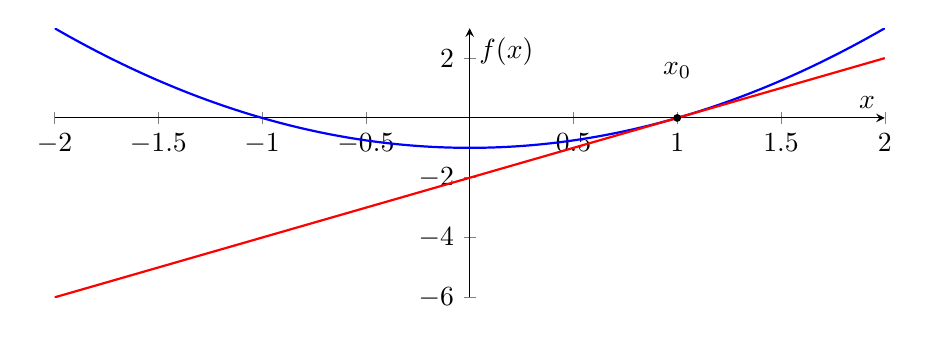
\begin{tikzpicture}
        \begin{axis}[
          axis lines=middle,
          xlabel={$x$},
          ylabel={$f(x)$},
          xtick={},
          ytick={},
          grid=none,
          width=\textwidth,
          height=5cm,
          domain=-2:2,
          samples=100
        ]
          \addplot[blue, thick] {x^2 - 1};
          % Tangent at point 1
          \addplot[red, thick, domain=-2:2] {2*x - 2};
          % Add point x_0
          \node at (axis cs:1,-0) [circle, fill=black, inner sep=1pt] {};
          \node at (axis cs:1,1) [above] {$x_0$};
        \end{axis}
      \end{tikzpicture}
    \end{column}
    \begin{column}{0.45\textwidth}
      \begin{block}{Definition}
        The derivative of a function $f:\mathbb{R}\to\mathbb{R}$ at a point $x_0$ is defined as:
        $$f'(x_0) = \lim_{h\to 0} \frac{f(x_0 + h) - f(x_0)}{h}$$
      \end{block}
      $\rightarrow$ The derivative represents the slope of the tangent line to the curve at the point $(x_0, f(x_0))$.
    \end{column}
  \end{columns}

  Usually computed thanks to product and chain rules:
  \begin{itemize}
    \item Product rule: $(uv)' = u'v + uv'$
    \item Chain rule: $(f(g(x)))' = f'(g(x))g'(x)$
  \end{itemize}
\end{frame}

\subsection{Extension to Multivariate setup: $f:\mathbb{R}^d \to \mathbb{R}$}

\begin{frame}{Limits and Continuity}
  \begin{block}{Open disk}
    An open disk of radius $\epsilon > 0$ centered at a point $\mathbf{x}_0 \in \mathbb{R}^d$ is defined as:
    $$\mathcal{B}(\mathbf{x}_0, \epsilon) = \{\mathbf{x} \in \mathbb{R}^d : \|\mathbf{x} - \mathbf{x}_0\|_2 < \epsilon\}$$
  \end{block}

  \begin{block}{Limit}
    The limit of a function $f:\mathbb{R}^d \to \mathbb{R}$ at a point $\mathbf{x}_0$ is defined as:
    $$\lim_{\mathbf{x} \to \mathbf{x}_0} f(\mathbf{x}) = L$$
    if $\forall \epsilon > 0, \exists \delta > 0$ such that if $\|\mathbf{x} - \mathbf{x}_0\|_2 < \delta$, then $|f(\mathbf{x}) - L| < \epsilon$.
  \end{block}

  A function is continuous at a point $\mathbf{x}_0$ if $\lim_{\mathbf{x} \to \mathbf{x}_0} f(\mathbf{x}) = f(\mathbf{x}_0)$.
\end{frame}

\begin{frame}{Directional derivative}

  \begin{block}{Directional derivative}
    The directional derivative of a function $f:\mathbb{R}^d \to \mathbb{R}$ at a point $\mathbf{x}_0$ in the direction of a vector $\mathbf{v} \in \mathbb{R}^d$ is defined as:
    $$Df(\mathbf{x}_0)[\mathbf{v}] = \lim_{h \to 0} \frac{f(\mathbf{x}_0 + h\mathbf{v}) - f(\mathbf{x}_0)}{h}$$
  \end{block}

  If $\|\mathbf{v}\|_2 = 1$, then $Df(\mathbf{x}_0)[\mathbf{v}]$ represents the rate of change of $f$ in the direction of $\mathbf{v}$ at the point $\mathbf{x}_0$.
 
  \textbf{Note :} We use alternatively the notation $\nabla_{\mathbf{v}}f(\mathbf{x}_0)$ for the directional derivative.

\end{frame}

\begin{frame}{Illustration of directional derivative}

  \begin{figure}[h]
    \centering
    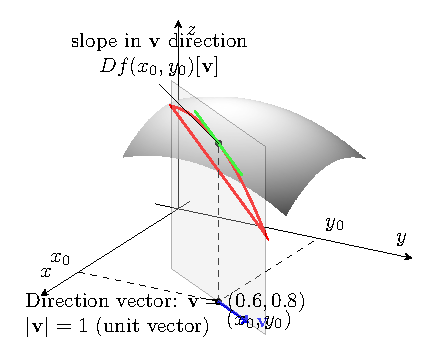
\includegraphics[height=\textheight]{figures/directional_derivative.pdf}
  \end{figure}

\end{frame}


\begin{frame}{Gradient}

  \begin{block}{Gradient}
    The gradient of a function $f:\mathbb{R}^d \to \mathbb{R}$ at a point $\mathbf{x}_0$ is defined as the vector of all directional derivatives in the standard basis directions:
    $$\nabla f(\mathbf{x}_0) = \left( Df(\mathbf{x}_0)[\mathbf{e}_1], Df(\mathbf{x}_0)\mathbf{e}_1, \ldots, Df(\mathbf{x}_0)\mathbf{e}_1 \right)^\mathrm{T}$$
    where $\{\mathbf{e}_1, \ldots, \mathbf{e}_d\}$ is the standard basis of $\mathbb{R}^d$.
  \end{block}

  $\rightarrow$ the direction of the steepest ascent of the function $f$ at the point $\mathbf{x}_0$.

  \begin{block}{Relationship with directional derivative}
    For any vector $\mathbf{v} \in \mathbb{R}^d$, the directional derivative can be expressed as:
    $$Df(\mathbf{x}_0)[\mathbf{v}] = \nabla f(\mathbf{x}_0)^\mathrm{T} \mathbf{v}$$
  \end{block}

\end{frame}
    

\begin{frame}{Graident and partial derivatives}

  \begin{block}{Partial derivatives}
    The partial derivative of a function $f:\mathbb{R}^d \to \mathbb{R}$ with respect to the $i$-th variable is defined as:
    $$\frac{\partial f}{\partial x_i}(\mathbf{x}_0) = \lim_{h \to 0} \frac{f(\mathbf{x}_0 + h\mathbf{e}_i) - f(\mathbf{x}_0)}{h}$$
    where $\mathbf{e}_i$ is the $i$-th standard basis vector.
  \end{block}

  The gradient can be expressed in terms of partial derivatives as:
  $$\nabla f(\mathbf{x}_0) = \left( \frac{\partial f}{\partial x_1}(\mathbf{x}_0), \frac{\partial f}{\partial x_2}(\mathbf{x}_0), \ldots, \frac{\partial f}{\partial x_d}(\mathbf{x}_0) \right)^\mathrm{T}$$

  $\rightarrow$ The gradient is a vector containing all the partial derivatives of the function at the point $\mathbf{x}_0$.
\end{frame}


\begin{frame}{Gradient properties and practical computation}

  \begin{block}{Derivative of a prodct}
    Let $g:\mathbb{R}^d \to \mathbb{R}$ and $h:\mathbb{R}^d \to \mathbb{R}$ be two functions. Then the gradient of their product $f(\mathbf{x}) = g(\mathbf{x})h(\mathbf{x})$ can be computed using the product rule:
    $$\nabla f(\mathbf{x}) = g(\mathbf{x})\nabla h(\mathbf{x}) + h(\mathbf{x})\nabla g(\mathbf{x})$$
  \end{block}

  \begin{block}{Derivative of a composition}
    Two cases:
    \begin{itemize}
      \item $f=h\circ g$ with: $h:\mathbb{R}\mapsto\mathbb{R}$ and $g:\mathbb{R}^d\mapsto\mathbb{R}$. The gradient of $f$ can be computed using the chain rule:
        $\nabla f(\mathbf{x}) = h'(g(\mathbf{x}))\nabla g(\mathbf{x})$, where $h'$ is the derivative of $h$.
      \item $f=h\circ g$ with: $h:\mathbb{R}^d\mapsto\mathbb{R}$ and $g:\mathbb{R}^{d'}\mapsto\mathbb{R}^d$. (We look at that later)
    \end{itemize}
  \end{block}
\end{frame}



\begin{frame}{Hessian matrix}

  \begin{block}{Hessian matrix}
    The Hessian matrix of a function $f:\mathbb{R}^d \to \mathbb{R}$ at a point $\mathbf{x}_0$ is defined as the square matrix of second-order partial derivatives:
    $$\mathbf{H}(\mathbf{x}_0) = \begin{pmatrix}
      \frac{\partial^2 f}{\partial x_1^2}(\mathbf{x}_0) & \frac{\partial^2 f}{\partial x_1 \partial x_2}(\mathbf{x}_0) & \cdots & \frac{\partial^2 f}{\partial x_1 \partial x_d}(\mathbf{x}_0) \\
      \frac{\partial^2 f}{\partial x_2 \partial x_1}(\mathbf{x}_0) & \frac{\partial^2 f}{\partial x_2^2}(\mathbf{x}_0) & \cdots & \frac{\partial^2 f}{\partial x_2 \partial x_d}(\mathbf{x}_0) \\
      \vdots & \vdots & \ddots & \vdots \\
      \frac{\partial^2 f}{\partial x_d \partial x_1}(\mathbf{x}_0) & \frac{\partial^2 f}{\partial x_d \partial x_2}(\mathbf{x}_0) & \cdots & \frac{\partial^2 f}{\partial x_d^2}(\mathbf{x}_0)
    \end{pmatrix}$$
  \end{block}

  $\rightarrow$ The Hessian matrix provides information about the curvature of the function $f$ at the point $\mathbf{x}_0$.
\end{frame}


\begin{frame}{Exercices}
  \begin{block}{Exercices}
    \begin{itemize}
      \item Compute the gradient and Hessian matrix of the function $f(x,y) = x^2 + 3xy + y^2$ at the point $(1,2)$.
      \item Using chain-rule compute gradient of $f(\mathbf{x}) = (\sum_i^{d}x_i^2)^(1/2)$.
    \end{itemize}
  \end{block}
\end{frame}


\begin{frame}{Hessian matrix properties}

  \begin{block}{Properties of the Hessian matrix}
    \begin{itemize}
      \item The Hessian is symmetric: $\mathbf{H}(\mathbf{x}_0) = \mathbf{H}(\mathbf{x}_0)^\mathrm{T}$.
      \item If $f$ is twice continuously differentiable, then the mixed partial derivatives are equal: $\frac{\partial^2 f}{\partial x_i \partial x_j} = \frac{\partial^2 f}{\partial x_j \partial x_i}$.
      \item The eigenvalues of the Hessian provide information about the local curvature of the function:
        \begin{itemize}
          \item If all eigenvalues are positive, $f$ is locally convex at $\mathbf{x}_0$.
          \item If all eigenvalues are negative, $f$ is locally concave at $\mathbf{x}_0$.
          \item If some eigenvalues are positive and others are negative, $f$ has a saddle point at $\mathbf{x}_0$.
        \end{itemize}
    \end{itemize}
  \end{block}
\end{frame}


\begin{frame}{Exercice}

  \begin{block}{Rosenbrock function}
    The Rosenbrock function is defined as:
    $$f(x,y) = (a - x)^2 + b(y - x^2)^2$$
    where $a$ and $b$ are constants (commonly $a=1$ and $b=100$).

    \begin{itemize}
      \item Compute the gradient $\nabla f(x,y)$. And find stationary point(s).
      \item Compute the Hessian matrix $\mathbf{H}(x,y)$. Analyse local curvature at the stationary point(s).
    \end{itemize}
  \end{block}
  
\end{frame}
  

\subsection{Multivariate case: $f:\mathbb{R}^d \to \mathbb{R}^p$}

\begin{frame}{Multivariate functions}
  \begin{block}{Multivariate function}
    A function $f:\mathbb{R}^d \to \mathbb{R}^p$ maps a vector $\mathbf{x} \in \mathbb{R}^d$ to a vector $\mathbf{y} \in \mathbb{R}^p$. We can write:
    $$f(\mathbf{x}) = \begin{pmatrix}
      f_1(\mathbf{x}) \\
      f_2(\mathbf{x}) \\
      \vdots \\
      f_p(\mathbf{x})
    \end{pmatrix}$$
  \end{block}
  The function $f$ is said to be vector-valued, and each component $f_i:\mathbb{R}^d \to \mathbb{R}$ is a scalar function.
\end{frame}

\begin{frame}{Gradient and Jacobian}
  \begin{block}{Gradient}
    The gradient of a function $f:\mathbb{R}^d \to \mathbb{R}$ is defined as:
    $$\nabla f(\mathbf{x}) = \left( \frac{\partial f}{\partial x_1}, \frac{\partial f}{\partial x_2}, \ldots, \frac{\partial f}{\partial x_d} \right)^\mathrm{T} \in \mathbb{R}^d$$
  \end{block}
  \begin{block}{Jacobian matrix}
    The Jacobian matrix of a function $f:\mathbb{R}^d \to \mathbb{R}^p$ is defined as:
    $$\mathbf{J}_f(\mathbf{x}) = \begin{pmatrix}
      \frac{\partial f_1}{\partial x_1} & \frac{\partial f_1}{\partial x_2} & \cdots & \frac{\partial f_1}{\partial x_d} \\
      \frac{\partial f_2}{\partial x_1} & \frac{\partial f_2}{\partial x_2} & \cdots & \frac{\partial f_2}{\partial x_d} \\
      \vdots & \vdots & \ddots & \vdots \\
      \frac{\partial f_p}{\partial x_1} & \frac{\partial f_p}{\partial x_2} & \cdots & \frac{\partial f_p}{\partial x_d}
    \end{pmatrix} \in \mathbb{R}^{p \times d}$$
  \end{block}
  $\rightarrow$ The Jacobian matrix generalizes the concept of gradient to vector-valued functions.
\end{frame}

\begin{frame}{Jacobian and directional derivative}
  \begin{block}{Directional derivative}
    The directional derivative of a function $f:\mathbb{R}^d \to \mathbb{R}^p$ in the direction of a vector $\mathbf{v} \in \mathbb{R}^d$ is defined as:
    $$Df(\mathbf{x})[\mathbf{v}] = \mathbf{J}_f(\mathbf{x})\mathbf{v} = \begin{pmatrix} \nabla f_1(\mathbf{x})^T \mathbf{v} \\ \nabla f_2(\mathbf{x})^T \mathbf{v} \\ \vdots \\ \nabla f_p(\mathbf{x})^T \mathbf{v} \end{pmatrix} \in \mathbb{R}^p$$
  \end{block}
  The directional derivative gives the rate of change of the function $f$ for all components in the direction of $\mathbf{v}$ at the point $\mathbf{x}$.
\end{frame}

\begin{frame}{Chain rule for composition of functions}
  \begin{block}{General chain rule}
    If $f:\mathbb{R}^d \to \mathbb{R}^p$ and $g:\mathbb{R}^m \to \mathbb{R}^d$, then the composition $h = f \circ g : \mathbb{R}^m \to \mathbb{R}^p$ is defined as:
    $$h(\mathbf{y}) = f(g(\mathbf{y}))$$
    The Jacobian of $h$ can be computed using the chain rule:
    $$\mathbf{J}_h(\mathbf{y}) = \mathbf{J}_f(g(\mathbf{y})) \mathbf{J}_g(\mathbf{y})$$
    where $\mathbf{J}_h(\mathbf{y}) \in \mathbb{R}^{p \times m}$, $\mathbf{J}_f(g(\mathbf{y})) \in \mathbb{R}^{p \times d}$, and $\mathbf{J}_g(\mathbf{y}) \in \mathbb{R}^{d \times m}$.
  \end{block}
\end{frame}

\begin{frame}{Chain rule: Special cases}
  \begin{block}{Case 1: $f:\mathbb{R}^d \to \mathbb{R}$ and $g:\mathbb{R}^m \to \mathbb{R}^d$}
    For $h = f \circ g : \mathbb{R}^m \to \mathbb{R}$, we have:
    $$\nabla h(\mathbf{y}) = \mathbf{J}_g(\mathbf{y})^T \nabla f(g(\mathbf{y}))$$
    where $\mathbf{J}_g(\mathbf{y}) \in \mathbb{R}^{d \times m}$ and $\nabla f(g(\mathbf{y})) \in \mathbb{R}^d$.
  \end{block}
  
  \begin{block}{Case 2: $f:\mathbb{R} \to \mathbb{R}$ and $g:\mathbb{R}^m \to \mathbb{R}$}
    For $h = f \circ g : \mathbb{R}^m \to \mathbb{R}$, we have:
    $$\nabla h(\mathbf{y}) = f'(g(\mathbf{y})) \nabla g(\mathbf{y})$$
    where $f'(g(\mathbf{y})) \in \mathbb{R}$ is a scalar and $\nabla g(\mathbf{y}) \in \mathbb{R}^m$.
  \end{block}
\end{frame}

\begin{frame}{Exercise 1: Basic Chain Rule}
  \begin{block}{Problem}
    Given:
    \begin{itemize}
      \item $f(\mathbf{x}) = \mathbf{x}^T\mathbf{x}$ where $f: \mathbb{R}^2 \to \mathbb{R}$
      \item $g(\mathbf{y}) = \begin{pmatrix} y_1 + y_2 \\ y_1 - y_2 \end{pmatrix}$ where $g: \mathbb{R}^2 \to \mathbb{R}^2$
      \item $h = f \circ g$
    \end{itemize}
    \vspace{0.3cm}
    \textbf{Task:} Find $\nabla h(\mathbf{y})$ using the chain rule.
  \end{block}
  
  \begin{block}{Chain Rule Formula (Case 1)}
    For $h = f \circ g$ where $f: \mathbb{R}^n \to \mathbb{R}$ and $g: \mathbb{R}^m \to \mathbb{R}^n$:
    $$\nabla h(\mathbf{y}) = \mathbf{J}_g(\mathbf{y})^T \nabla f(g(\mathbf{y}))$$
  \end{block}
\end{frame}

\begin{frame}{Exercise 1: Solution}
  \begin{block}{Step 1: Compute $\nabla f(\mathbf{x})$}
    Using matrix calculus: $f(\mathbf{x}) = \mathbf{x}^T\mathbf{x}$
    $$\nabla f(\mathbf{x}) = 2\mathbf{x}$$
  \end{block}
  
  \begin{block}{Step 2: Compute Jacobian $\mathbf{J}_g(\mathbf{y})$}
    $$g(\mathbf{y}) = \begin{pmatrix} y_1 + y_2 \\ y_1 - y_2 \end{pmatrix} \Rightarrow \mathbf{J}_g(\mathbf{y}) = \begin{pmatrix} 1 & 1 \\ 1 & -1 \end{pmatrix}$$
  \end{block}
  
  \begin{block}{Step 3: Apply chain rule}
    $$\nabla h(\mathbf{y}) = \mathbf{J}_g(\mathbf{y})^T \nabla f(g(\mathbf{y})) = \begin{pmatrix} 1 & 1 \\ 1 & -1 \end{pmatrix} \cdot 2g(\mathbf{y})$$
    $$= 2\begin{pmatrix} 1 & 1 \\ 1 & -1 \end{pmatrix}\begin{pmatrix} y_1 + y_2 \\ y_1 - y_2 \end{pmatrix} = 2\begin{pmatrix} 2y_1 \\ 2y_2 \end{pmatrix} = \begin{pmatrix} 4y_1 \\ 4y_2 \end{pmatrix}$$
  \end{block}
\end{frame}

\begin{frame}{Exercise 1: Verification}
  \begin{block}{Direct computation}
    $$h(\mathbf{y}) = f(g(\mathbf{y})) = (y_1 + y_2)^2 + (y_1 - y_2)^2$$
    $$= y_1^2 + 2y_1y_2 + y_2^2 + y_1^2 - 2y_1y_2 + y_2^2 = 2y_1^2 + 2y_2^2$$
    
    Therefore:
    $$\nabla h(\mathbf{y}) = \begin{pmatrix} 4y_1 \\ 4y_2 \end{pmatrix} \quad \checkmark$$
  \end{block}
\end{frame}

\begin{frame}{Exercise 2: General Quadratic Forms}
  \begin{block}{Problem (General Case)}
    Given:
    \begin{itemize}
      \item $f(\mathbf{x}) = \mathbf{x}^T\mathbf{A}\mathbf{x} + \mathbf{b}^T\mathbf{x}$ where $f: \mathbb{R}^n \to \mathbb{R}$
      \item $\mathbf{A} \in \mathbb{R}^{n \times n}$ symmetric, $\mathbf{b} \in \mathbb{R}^n$
      \item $g(\mathbf{y}) = \mathbf{C}\mathbf{y}$ where $g: \mathbb{R}^m \to \mathbb{R}^n$
      \item $\mathbf{C} \in \mathbb{R}^{n \times m}$
      \item $h = f \circ g$
    \end{itemize}
    \vspace{0.3cm}
    \textbf{Task:} Find $\nabla h(\mathbf{y})$ using matrix calculus and the chain rule.
  \end{block}
  
  \begin{block}{Matrix Calculus Rules}
    \begin{itemize}
      \item $\nabla(\mathbf{x}^T\mathbf{A}\mathbf{x}) = 2\mathbf{A}\mathbf{x}$ (when $\mathbf{A}$ symmetric)
      \item $\nabla(\mathbf{b}^T\mathbf{x}) = \mathbf{b}$
      \item For linear $g(\mathbf{y}) = \mathbf{C}\mathbf{y}$: $\mathbf{J}_g(\mathbf{y}) = \mathbf{C}$
    \end{itemize}
  \end{block}
\end{frame}

\begin{frame}{Exercise 2: General Solution}
  \begin{block}{Step 1: Compute $\nabla f(\mathbf{x})$}
    Using matrix calculus rules:
    $$\nabla f(\mathbf{x}) = 2\mathbf{A}\mathbf{x} + \mathbf{b}$$
  \end{block}
  
  \begin{block}{Step 2: Compute Jacobian $\mathbf{J}_g(\mathbf{y})$}
    Since $g(\mathbf{y}) = \mathbf{C}\mathbf{y}$ (linear transformation):
    $$\mathbf{J}_g(\mathbf{y}) = \mathbf{C} \in \mathbb{R}^{n \times m}$$
  \end{block}
  
  \begin{block}{Step 3: Apply chain rule}
    $$\nabla h(\mathbf{y}) = \mathbf{J}_g(\mathbf{y})^T \nabla f(g(\mathbf{y}))$$
    $$= \mathbf{C}^T [2\mathbf{A}(\mathbf{C}\mathbf{y}) + \mathbf{b}]$$
    $$= 2\mathbf{C}^T\mathbf{A}\mathbf{C}\mathbf{y} + \mathbf{C}^T\mathbf{b}$$
  \end{block}
\end{frame}


\begin{frame}{Exercise 2: Numerical Example}
  \begin{block}{Specific case: $n=3, m=2$}
    \begin{itemize}
      \item $\mathbf{A} = \begin{pmatrix} 2 & 0 & 1 \\ 0 & 1 & 0 \\ 1 & 0 & 3 \end{pmatrix}$, $\mathbf{b} = \begin{pmatrix} 1 \\ -1 \\ 2 \end{pmatrix}$
      \item $\mathbf{C} = \begin{pmatrix} 1 & 2 \\ 0 & 1 \\ 1 & 0 \end{pmatrix}$
    \end{itemize}
    
    Computing the required matrices:
    $$\mathbf{C}^T\mathbf{A}\mathbf{C} = \begin{pmatrix} 1 & 0 & 1 \\ 2 & 1 & 0 \end{pmatrix}\begin{pmatrix} 2 & 0 & 1 \\ 0 & 1 & 0 \\ 1 & 0 & 3 \end{pmatrix}\begin{pmatrix} 1 & 2 \\ 0 & 1 \\ 1 & 0 \end{pmatrix} = \begin{pmatrix} 7 & 6 \\ 6 & 9 \end{pmatrix}$$
    
    $$\mathbf{C}^T\mathbf{b} = \begin{pmatrix} 1 & 0 & 1 \\ 2 & 1 & 0 \end{pmatrix}\begin{pmatrix} 1 \\ -1 \\ 2 \end{pmatrix} = \begin{pmatrix} 3 \\ 1 \end{pmatrix}$$
    
    Therefore:
    $$\nabla h(\mathbf{y}) = 2\begin{pmatrix} 7 & 6 \\ 6 & 9 \end{pmatrix}\mathbf{y} + \begin{pmatrix} 3 \\ 1 \end{pmatrix} = \begin{pmatrix} 14y_1 + 12y_2 + 3 \\ 12y_1 + 18y_2 + 1 \end{pmatrix}$$
  \end{block}
\end{frame}

\begin{frame}{Key Takeaways}
  \begin{block}{Advantages of Matrix Calculus Approach}
    \begin{itemize}
      \item \textbf{Scalability:} Works for arbitrary dimensions without modification
      \item \textbf{Efficiency:} No component-wise partial derivatives needed
      \item \textbf{Clarity:} Clean matrix operations instead of summations
      \item \textbf{Generality:} Same formulas apply regardless of problem size
    \end{itemize}
  \end{block}
  
  \begin{block}{General Chain Rule Pattern}
    For compositions $h = f \circ g$:
    \begin{enumerate}
      \item Identify the structure of $f$ and $g$
      \item Use appropriate matrix calculus rules for $\nabla f$ and $\mathbf{J}_g$
      \item Apply: $\nabla h(\mathbf{y}) = \mathbf{J}_g(\mathbf{y})^T \nabla f(g(\mathbf{y}))$
      \item Verify using direct computation when possible
    \end{enumerate}
  \end{block}
\end{frame}

\subsection{Matrix functions: $f:\mathbb{R}^{m,n} \to \mathbb{R}$}

\begin{frame}{Fréchet derivative -- Definition}
  \begin{block}{Fréchet differentiability}
    A function $f:\mathbb{R}^{m \times n}\to\mathbb{R}^{p \times q}$ is differentiable at $\mathbf{X}$ if there exists a linear mapping $Df(\mathbf{X}):\mathbb{R}^{m \times n}\to\mathbb{R}^{p \times q}$ such that
    $$\lim_{\|\mathbf{V}\|_F\to 0} \frac{\|f(\mathbf{X}+\mathbf{V}) - f(\mathbf{X}) - Df(\mathbf{X})[\mathbf{V}]\|_F}{\|\mathbf{V}\|_F} = 0$$\\
    $\mathbf{D} f(\mathbf{X})[\boldsymbol{\xi}] = f(\mathbf{X}+\mathbf{\xi}) - f(\mathbf{X}) + o(\lVert\boldsymbol{\xi}\rVert)$
  \end{block}
  
  \begin{block}{Gateaux derivative (alternative characterization)}
    If $f$ is Fréchet differentiable at $\mathbf{X}$, then for any $\mathbf{V}$:
    $$Df(\mathbf{X})[\mathbf{V}] = \left.\frac{d}{dt}\right|_{t=0} f(\mathbf{X}+t\mathbf{V}) = \lim_{t\to 0} \frac{f(\mathbf{X}+t\mathbf{V}) - f(\mathbf{X})}{t}$$
  \end{block}
  
  \textbf{Note:} If $\left.\frac{d}{dt}\right|_{t=0} f(\mathbf{X}+t\mathbf{V})$ is not linear in $\mathbf{V}$, then $f$ is not Fréchet differentiable.
\end{frame}

\begin{frame}{What it means to derive a matrix function?}
  \begin{block}{Matrix function}
    A matrix function $f:\mathbb{R}^{m,n} \to \mathbb{R}$ maps a matrix $\mathbf{X} \in \mathbb{R}^{m,n}$ to a scalar value. For example, $f(\mathbf{X}) = \|\mathbf{X}\|_F^2$.
  \end{block}
  
  \begin{block}{Directional derivative}
    The directional derivative of $f$ at $\mathbf{X}$ in direction $\mathbf{V}$ is:
    $$Df(\mathbf{X})[\mathbf{V}] = \lim_{h \to 0} \frac{f(\mathbf{X} + h\mathbf{V}) - f(\mathbf{X})}{h}$$
    where $\mathbf{V} \in \mathbb{R}^{m,n}$ is a perturbation matrix.
  \end{block}
  
  Since $Df(\mathbf{X})$ is linear, it can be represented using the gradient matrix.
\end{frame}
  
\begin{frame}{Gradient in the matrix to scalar case}
  \begin{block}{Gradient definition}
    For $f:\mathbb{R}^{m,n} \to \mathbb{R}$, the gradient $\nabla f(\mathbf{X}) \in \mathbb{R}^{m,n}$ satisfies:
    $$Df(\mathbf{X})[\mathbf{V}] = \mathrm{Tr}(\nabla f(\mathbf{X})^\mathrm{T} \mathbf{V})$$
    where $\mathrm{Tr}(\cdot)$ denotes the trace of a matrix.
  \end{block}
  
  \begin{block}{Link to partial derivatives}
    The gradient can be computed using partial derivatives:
    $$\nabla f(\mathbf{X}) = \begin{pmatrix}
      \frac{\partial f}{\partial X_{11}} & \frac{\partial f}{\partial X_{12}} & \cdots & \frac{\partial f}{\partial X_{1n}} \\
      \frac{\partial f}{\partial X_{21}} & \frac{\partial f}{\partial X_{22}} & \cdots & \frac{\partial f}{\partial X_{2n}} \\
      \vdots & \vdots & \ddots & \vdots \\
      \frac{\partial f}{\partial X_{m1}} & \frac{\partial f}{\partial X_{m2}} & \cdots & \frac{\partial f}{\partial X_{mn}}
    \end{pmatrix}$$
  \end{block}
\end{frame}

\begin{frame}{Examples: Matrix to scalar functions}
  \textbf{Example 1:} $f(\mathbf{X}) = \|\mathbf{X}\|_F^2 = \mathrm{Tr}(\mathbf{X}^\mathrm{T}\mathbf{X})$
  
  Using Gateaux derivative:
  $$Df(\mathbf{X})[\mathbf{V}] = \left.\frac{d}{dt}\right|_{t=0} \mathrm{Tr}((\mathbf{X}+t\mathbf{V})^\mathrm{T}(\mathbf{X}+t\mathbf{V}))$$
  $$= \left.\frac{d}{dt}\right|_{t=0} [\mathrm{Tr}(\mathbf{X}^\mathrm{T}\mathbf{X}) + 2t\mathrm{Tr}(\mathbf{X}^\mathrm{T}\mathbf{V}) + t^2\mathrm{Tr}(\mathbf{V}^\mathrm{T}\mathbf{V})]$$
  $$= 2\mathrm{Tr}(\mathbf{X}^\mathrm{T}\mathbf{V})$$
  
  Therefore: $\boxed{\nabla f(\mathbf{X}) = 2\mathbf{X}}$
  
  \vspace{10pt}
  
  \textbf{Example 2:} $f(\mathbf{X}) = \log\det(\mathbf{X})$ (for invertible $\mathbf{X}$)
  
  $$Df(\mathbf{X})[\mathbf{V}] = \left.\frac{d}{dt}\right|_{t=0} \log\det(\mathbf{X}+t\mathbf{V}) = \mathrm{Tr}(\mathbf{X}^{-1}\mathbf{V})$$
  
  Therefore: $\boxed{\nabla f(\mathbf{X}) = \mathbf{X}^{-\mathrm{T}}}$
\end{frame}

\subsection{Matrix functions: $f:\mathbb{R}^{m,n} \to \mathbb{R}^{p,q}$}

\begin{frame}{Matrix to matrix functions}
  \begin{block}{Matrix-valued function}
    A function $f:\mathbb{R}^{m,n} \to \mathbb{R}^{p,q}$ maps a matrix $\mathbf{X} \in \mathbb{R}^{m,n}$ to a matrix $\mathbf{Y} \in \mathbb{R}^{p,q}$.
  \end{block}
  
  \begin{block}{Directional derivative}
    The directional derivative $Df(\mathbf{X})[\mathbf{V}]$ is a linear mapping from $\mathbb{R}^{m,n}$ to $\mathbb{R}^{p,q}$:
    $$Df(\mathbf{X})[\mathbf{V}] = \lim_{t \to 0} \frac{f(\mathbf{X} + t\mathbf{V}) - f(\mathbf{X})}{t}$$
  \end{block}
  
  \begin{block}{Vectorization representation}
    Since $Df(\mathbf{X})$ is linear, there exists a matrix $\mathbf{M}_{\mathbf{X}} \in \mathbb{R}^{pq \times mn}$ such that:
    $$\mathrm{vec}(Df(\mathbf{X})[\mathbf{V}]) = \mathbf{M}_{\mathbf{X}} \mathrm{vec}(\mathbf{V})$$
    where $\mathrm{vec}(\cdot)$ stacks matrix columns into a vector.
  \end{block}
\end{frame}

\begin{frame}{Vectorization identities}
  \begin{block}{Key identities for matrix calculus}
    \begin{itemize}
      \item $\mathrm{vec}(\mathbf{A}\mathbf{B}\mathbf{C}) = (\mathbf{C}^\mathrm{T} \otimes \mathbf{A}) \mathrm{vec}(\mathbf{B})$
      \item $\mathrm{Tr}(\mathbf{A}\mathbf{B}) = \mathrm{vec}(\mathbf{A})^\mathrm{T}\mathrm{vec}(\mathbf{B})$
      \item $\mathrm{Tr}(\mathbf{A}^\mathrm{T}\mathbf{B}) = \mathrm{vec}(\mathbf{A})^\mathrm{T}\mathrm{vec}(\mathbf{B})$
    \end{itemize}
  \end{block}
  
  where $\otimes$ denotes the Kronecker product.
  
  \vspace{10pt}
  
  These identities allow us to:
  \begin{itemize}
    \item Convert matrix operations to vector operations
    \item Find the matrix $\mathbf{M}_{\mathbf{X}}$ in the vectorization representation
    \item Compute derivatives efficiently
  \end{itemize}
\end{frame}

\begin{frame}{Examples: Matrix to matrix functions}
  \textbf{Example 1:} $f(\mathbf{X}) = \mathbf{X}^2$
  
  Using Gateaux derivative:
  $$Df(\mathbf{X})[\mathbf{V}] = \left.\frac{d}{dt}\right|_{t=0} (\mathbf{X}+t\mathbf{V})^2$$
  $$= \left.\frac{d}{dt}\right|_{t=0} [\mathbf{X}^2 + t(\mathbf{X}\mathbf{V} + \mathbf{V}\mathbf{X}) + t^2\mathbf{V}^2]$$
  $$= \mathbf{X}\mathbf{V} + \mathbf{V}\mathbf{X}$$
  
  Therefore: $\boxed{Df(\mathbf{X})[\mathbf{V}] = \mathbf{X}\mathbf{V} + \mathbf{V}\mathbf{X}}$
  
  \vspace{10pt}
  
  \textbf{Example 2:} $f(\mathbf{X}) = \mathbf{X}^{-1}$ (for invertible $\mathbf{X}$)
  
  From the identity $\mathbf{X}\mathbf{X}^{-1} = \mathbf{I}$ and product rule:
  $$\mathbf{V}\mathbf{X}^{-1} + \mathbf{X} \, Df(\mathbf{X})[\mathbf{V}] = \mathbf{0}$$
  
  Therefore: $\boxed{Df(\mathbf{X})[\mathbf{V}] = -\mathbf{X}^{-1}\mathbf{V}\mathbf{X}^{-1}}$
\end{frame}

\begin{frame}{Properties of matrix function derivatives}
  \begin{block}{Linearity}
    For $f = \alpha g + \beta h$:
    $$Df(\mathbf{X})[\mathbf{V}] = \alpha \, Dg(\mathbf{X})[\mathbf{V}] + \beta \, Dh(\mathbf{X})[\mathbf{V}]$$
  \end{block}
  
  \begin{block}{Product rule}
    For $f(\mathbf{X}) = g(\mathbf{X}) \cdot h(\mathbf{X})$ (matrix multiplication):
    $$Df(\mathbf{X})[\mathbf{V}] = Dg(\mathbf{X})[\mathbf{V}] \cdot h(\mathbf{X}) + g(\mathbf{X}) \cdot Dh(\mathbf{X})[\mathbf{V}]$$
  \end{block}
  
  \begin{block}{Chain rule}
    For $f(\mathbf{X}) = g(h(\mathbf{X}))$:
    $$Df(\mathbf{X})[\mathbf{V}] = Dg(h(\mathbf{X}))[Dh(\mathbf{X})[\mathbf{V}]]$$
  \end{block}
\end{frame}

\begin{frame}{Chain rule example}
  \textbf{Example:} $f(\mathbf{X}) = (\mathbf{X}^{1/2})^2 = \mathbf{X}$
  
  Let $g(\mathbf{Y}) = \mathbf{Y}^2$ and $h(\mathbf{X}) = \mathbf{X}^{1/2}$, so $f(\mathbf{X}) = g(h(\mathbf{X}))$.
  
  We know:
  \begin{itemize}
    \item $Dg(\mathbf{Y})[\mathbf{W}] = \mathbf{Y}\mathbf{W} + \mathbf{W}\mathbf{Y}$
    \item $Df(\mathbf{X})[\mathbf{V}] = \mathbf{V}$ (since $f(\mathbf{X}) = \mathbf{X}$)
  \end{itemize}
  
  Using the chain rule:
  $$Df(\mathbf{X})[\mathbf{V}] = Dg(h(\mathbf{X}))[Dh(\mathbf{X})[\mathbf{V}]]$$
  $$\mathbf{V} = \mathbf{X}^{1/2} \, Dh(\mathbf{X})[\mathbf{V}] + Dh(\mathbf{X})[\mathbf{V}] \, \mathbf{X}^{1/2}$$
  
  This gives us a Sylvester equation for $Dh(\mathbf{X})[\mathbf{V}]$:
  $$\mathbf{X}^{1/2} \, Dh(\mathbf{X})[\mathbf{V}] + Dh(\mathbf{X})[\mathbf{V}] \, \mathbf{X}^{1/2} = \mathbf{V}$$
\end{frame}

\begin{frame}{Summary: Matrix function differentiation}
  \begin{block}{Key concepts}
    \begin{itemize}
      \item \textbf{Fréchet derivative}: Captures linear approximation of matrix functions
      \item \textbf{Matrix-to-scalar}: Gradient $\nabla f(\mathbf{X})$ with $Df(\mathbf{X})[\mathbf{V}] = \mathrm{Tr}(\nabla f(\mathbf{X})^\mathrm{T} \mathbf{V})$
      \item \textbf{Matrix-to-matrix}: Linear operator $Df(\mathbf{X})$ with vectorization representation
      \item \textbf{Vectorization}: Converts matrix operations to linear algebra on vectors
    \end{itemize}
  \end{block}
  
  \begin{block}{Applications}
    \begin{itemize}
      \item Optimization on matrix manifolds
      \item Machine learning (gradient descent for matrix parameters)
      \item Sensitivity analysis
      \item Perturbation theory
    \end{itemize}
  \end{block}
\end{frame}

\end{document}


